\documentclass[12pt]{article}

\usepackage{sbc-template}

\usepackage{graphicx,url}

%\usepackage[brazil]{babel}
\usepackage[utf8]{inputenc} 

     
\sloppy

\title{A qualidade na engenharia de requisitos e sua contribuição para uma empresa de software}

\author{Renato M. Soares, Thiago L. Andrade}

\address{CIVT - Centro Integrado de Vocação Tecnológica\\
Universidade Federal do Rio Grande do Norte (UFRN)\\
Natal -- RN -- Brasil
\email{rmsnatal@gmail.com, thiago@limaandrade.com}
}

\begin{document} 

\maketitle
     
\begin{resumo} 
Este artigo apresenta algumas formas de se atingir melhores níveis de qualidade na 
engenharia de requisitos em processos de desenvolvimento de software. Para isso é 
apresentado motivos que comprovam a importância da etapa de requisitos em qualquer 
projeto de software, seguido dos atributos da qualidade em um documento de 
requisitos. é apresentado também um estudo de caso de uma empresa de desenvolvimento 
de software para se exemplificar como o documento de requisitos é importante nas 
diversas fases do desenvolvimento de um produto de software e quais as implicações 
que podem ocorrer devido a falta de qualidade nesse artefato. Por fim concluímos a 
problemática fazendo um balanço geral de todo que foi apresentado além de 
possíveis soluções.
\end{resumo}

\section{Introdução e motivação}
Um dos principais objetivos da qualidade de software é garantir um produto final 
de software que satisfaça o que foi acordado com o cliente, ou entre os interessados, 
num dado momento inicial desde as fases iniciais do projeto, várias medidas ou 
metodologias de otimização da qualidade de software podem ser aplicadas para as 
diferentes etapas de desenvolvimento adotadas por uma empresa.

Segundo a IEEE (Instituto de Engenheiros Eletricistas e Eletrônicos), a qualidade 
de software é definida como “o grau com que o sistema, componente ou processo atende 
aos requisitos especificados e às expectativas ou necessidades de clientes ou usuários”. 
Enquanto a ISO (em português: Organização Internacional de Normalização) define a 
qualidade como sendo “a totalidade de características de um produto ou serviço que 
comprovam sua capacidade de satisfazer necessidades especificadas ou implícitas”. 
Diante disso, temos definições que mostram que a qualidade de um produto está diretamente 
ligada aos seus requisitos inerentes.

Garantir que um sistema ou componente atenda ao que é esperado pelos clientes ou 
usuários está ligado ao conceito e definição do que vem a ser a Qualidade de Software, 
bem como, cabe ao sistema comprovar também que é capaz de satisfazer as necessidades 
especificadas e implícitas ao se ouvir a voz do cliente. Assim, é notório que a qualidade 
de um software tem uma relação direta com os requisitos levantados que devem ser atendidos.

O processo de desenvolvimento de um produto de software, de acordo com as metodologias de 
desenvolvimento mais utilizadas, tem início pela elicitação dos requisitos, sendo a etapa 
responsável por determinar os requisitos que o software deverá atender. Após essa etapa, 
temos a fase de modelagem e a de análise dos requisitos, que podem geram como artefato um 
documento de requisitos.

Por isso se faz relevante um estudo sobre como a qualidade em engenharia de requisitos 
pode ser um fator de importante contribuição para uma empresa de software. Nesse artigo 
estudaremos problemas enfrentados em uma empresa relacionados a uma má adequação a 
engenharia de requisitos.

\section{Atributos de qualidade em documentos de requisitos}

Segundo \cite{hofmann:2001} a engenharia de requisitos é uma das mais importantes 
partes de qualquer projeto de software e os responsáveis pelas práticas de engenharia de 
requisitos claramente contribuem para o sucesso do projeto, principalmente em termos de 
conhecimentos de times, alocação de recursos e processos. É perceptível então como a 
engenharia de requisitos afeta outras partes do desenvolvimento de software, ou seja, é 
uma forte candidata a interferir na qualidade de um produto de software.

Devido a importância da engenharia de requisitos, é aconselhável fazer uso de atributos
da qualidade para nesta parte do desenvolvimento de um projeto de software para que os 
resultados obtidos por uma engenharia de requisitos bem feita nas suas etapas de elicitação, 
validação e análise, por exemplo, gerem artefatos bem produzidos e com qualidade aplicada.

Sabe-se que o principal artefato gerado pela engenharia de requisitos é o documento de 
requisitos em si. Dependendo do modelo seguido, junto a este documento alguns artefatos 
poderão ser encontrados. Nesse sentido, analisar a qualidade de um documento de requisitos 
envolve avaliar a qualidade dos artefatos de software produzidos na engenharia de requisitos. 
Uma boa forma de se garantir qualidade em artefatos da engenharia de requisitos é por meio da 
implantação de inspeções que ajudam a encontrar defeitos nestes artefatos como uma forma 
preventiva para que ações futuras de outras etapas do desenvolvimento não usem artefatos 
problemáticos.

\section{Problemas decorrentes de falhas na engenharia de requisitos na empresa 
Sig Software & Consultoria}

A Sig Software & Consultoria “é uma empresa especializada na construção e implantação de 
sistemas de gestão. A empresa nasceu em 2011 a partir de um spin-off da UFRN onde o seus 
fundadores foram responsáveis pelo desenvolvimento e implantação dos sistemas SIG na 
instituição.” \cite{esig:2014}. A partir dela, abordaremos um estudo de caso sobre os problemas 
inerentes ao processo de criação e manutenção de documentos de requisitos, e suas 
consequências para o processo de desenvolvimento como um todo.

Na SIG Software é adotado o processo de desenvolvimento ágil Scrum, tanto pelas equipes 
de desenvolvimento quanto as de testes, sendo todas elas compostas por um \textit{scrum master}, 
ou seja, o responsável pela sua equipe e o que lida com o papel de “guardião” da equipe 
no contexto da empresa. Por muitas vezes que é necessária a comunicação entre duas 
equipes, o guardião é encarregado de tomar decisões referentes às atividades da sua 
\textit{sprint}.

Além disso, os guardiões também são responsáveis por participar de reuniões com clientes, 
para assim, centralizar informações necessárias aos membros de suas equipes. Desde as 
reuniões de elicitação de requisitos até o momento de implantação e entrega do produto, 
são gerados e utilizados, como artefatos, vários documentos de requisitos.

Em cada etapa da construção e projeto do software é necessária a criação ou atualização 
de pelo menos um requisito, sendo que, por muitas vezes, isso não é feito na empresa. 
É comum se deparar com funcionalidades implementadas que não condiz com o que está 
especificado no documento de requisitos, ou até mesmo casos em que o documento 
não existe.

Em cada etapa da construção e projeto do software é necessária a criação ou atualização 
de pelo menos um documento. Por exemplo, na reunião de elicitação com o cliente, que visa 
captar informações sobre os requisitos que o cliente deseja, é gerado como artefato uma ata 
de reunião que, por sua vez, é utilizada para gerar o documento de requisitos. Ao ter os 
requisitos documentados, sendo até o momento um documento que representa, de alto nível, 
as necessidades dos clientes, o mesmo pode ser utilizado como espelho para a criação de 
outros documentos, como: casos de uso, diagramas de atividades, diagramas de sequência, 
entre outros. Com isso, podemos ver que tudo está diretamente ligado à documentos e 
estes, precisam ser constantemente atualizados conforme necessidades para evitar 
conflitos, quando dois documentos apresentam dados contraditórios, por exemplo, e para 
manter centralizadas e coerentes as informações de conhecimento da empresa e que são 
necessárias durante o projeto.

A atividade de atualização de documentos é de grande importância para todas as equipes 
da empresa e, principalmente, para as que lidam diretamente com a produção do código dos 
sistemas, como os desenvolvedores e testadores. Apesar disso, por muitas vezes, a atualização 
dos requisitos não é feita na empresa. É comum se deparar com funcionalidades implementadas que 
não condiz com o que está especificado nos documentos, ou até mesmo casos em que atividades 
produzidas não estão devidamente documentadas.

Tanto a carência de documentos quanto a existência de documentos não atualizados, causa 
atraso em todos os setores da empresa. Inerente a esse problema, a consequência principal é 
a falta de informação dos envolvidos, no momento de…

\section{Conclusão}

Importância de se aplicar atributos de qualidade, da existência e manutenção de 
documentos de requisitos para a melhoria da qualidade de software em geral.

\bibliographystyle{sbc}
\bibliography{referencias}

\end{document}

%FIGURA
%\begin{figure}[ht]
%\centering
%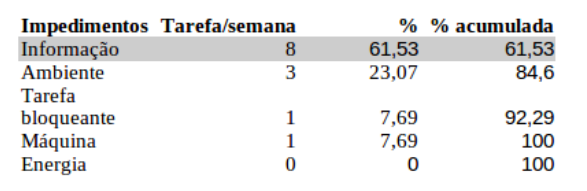
\includegraphics[width=.3\textwidth]{fig1.png}
%\caption{This figure is an example of a figure caption taking more than one
%line and justified considering margins mentioned in Section~\ref{sec:figs}.}
%\label{fig:exampleFig2}
%\end{figure}
